\documentclass{FR16} 
\begin{document}
\maketitle

\newpage

\section{ΕΙΣΑΓΩΓΗ}
Στο δεύτερο μέρος των ασκήσεων του μαθήματος μας δόθηκε σειριακός κώδικας που υπολόγιζε μια απλοποιημένη μορφή του ω statistic, όπως εμφανίζεται για ανίχνευση θετικής επιλογής σε ακολουθίες DNA. Ο στόχος μας ήταν η βελτιστοποίηση της απόδοσης αυτού του κώδικα με την χρήση διαφορετικών τεχνικών. Η βελτιστοποίηση υπήρξε σε πολλά διαφορετικά επίπεδα δηλαδή πρώτα από επίπεδο πυρήνα, σε επίπεδο επεξεργαστή και τέλος σε nodes. Για να επιτευχθεί αυτό έγινε χρήση των εργαλείων SSE,phtreads και MPI. Τέλος προσπαθήσαμε να βελτιώσουμε το memory layout για να πετύχουμε καλύτερη απόδοση για την υλοποίηση με SSE εντολές. Στο κομμάτι των pthread χρησιμοποιήσαμε σαν βάση τον κώδικα που μας δόθηκε από την προηγούμενη εργασία.
\newpage

\section{ΣΕΙΡΙΑΚΟΣ ΚΩΔΙΚΑΣ}
Ο αρχικός κώδικας που μας δόθηκε δέχεται ως είσοδο τον αριθμό των επαναλήψεων που μας καθορίζει το τελικό αποτέλεσμα του κωδικά μας. Αρχικά ξεκινάει και αρχικοποιεί τις μεταβλητές avgF,maxF,minF καθώς σε αυτές θα εκχωρήσουμε τα αποτελέσματα μας. Δεσμεύουμε την μνήμη με την χρήση της malloc για τα 6 arrays: mVec,nVec,Lvec,Rvec,Cvec και FVec και τα αρχικοποιούμαι με τυχαίες τιμές.Αμέσως μετά ακολουθεί ένα διπλό loop. Tο εσωτερικό for-loop είναι υπεύθυνο για το υπολογισμό των ω τιμών ενώ το εξωτερικό επαναλαμβάνει τους υπολογισμούς με σκοπό την πιο ακριβή μέτρηση βάση του μέσου όρου περισσότερων εκτελέσεων. 
Το πρόγραμμα έτρεξε με εξής αποτελέσματα και χρόνους.
\subsection{ΧΡΟΝΟΙ ΕΚΤΕΛΕΣΗΣ}
\begin{center}
\begin{tabular}{c c c}
\arrayrulecolor{Azzurro}
\hline
{\bfseries $Ν$} & {\bfseries $Omega time$} & {\bfseries $Total time$}\\
\hline
10    & 0.000001 & 0.000157 \\
100   & 0.000006 & 0.000189 \\
1000  & 0.000075 & 0.001307 \\
10000 & 0.000572 & 0.010063 \\
100000 & 0.001870 & 0.035958 \\
1000000 & 0.018978 & 0.299918 \\
10000000 & 0.187648 & 2.914389 \\
\hline
\end{tabular}
\end{center}

\subsection{ΑΠΟΤΕΛΕΣΜΑΤΑ}
\begin{center}
\begin{tabular}{c c c c}
\arrayrulecolor{Azzurro}
\hline
{\bfseries $Ν$} & {\bfseries $Min$} & {\bfseries $Max$} & {\bfseries $Average$}\\
\hline
10    & 1.757855e-02 & 4.314111e-01 & 1.809734e+00 \\
100   & -8.182857e+00 & 3.055697e+01 & 5.937088e+01 \\
1000  & -3.680385e+02 & 6.000032e+02 & 4.379610e+02 \\
10000 & -7.426174e+02 & 6.029684e+03 & 7.123071e+03 \\
100000 & -9.448395e+03 & 1.896388e+04 & 2.698570e+04  \\
1000000 & -1.110300e+05 & 2.169382e+05 & 3.659404e+05 \\
10000000 & -2.711918e+06 &  6.048419e+05 & -6.529043e+06 \\
\hline
\end{tabular}
\end{center}
\newpage

\section{SSE}
Στο πρώτα κομμάτι της δικής μας υλοποίησης, ο στόχος ήταν η κατά το δυνατόν βελτίωση της απόδοσης του σειριακού κώδικα, διατηρώντας τα αποτελέσματα αναλλοίωτα, με την χρήση της βιβλιοθήκης της C, SSE. Για να μπορέσουμε να χρησιμοποιήσουμε τον SSE κώδικα εισάγαμε τα libraries που ήταν απαραίτητα με την εντολή \textit{"xmmintrin.h"}.Το for-loop που μας ενδιαφέρει να βελτιστοποιήσουμε είναι αυτό που κάνει όλους τους απαραίτητους υπολογισμούς. Για να συμβεί όμως αυτό είναι απαραίτητες διάφορες αλλαγές στον κώδικά μας. Αρχικά πλέον δεν δεσμεύουμε την μνήμη με την χρήση της malloc αλλά με την χρήση της mmmalloc. Οι τιμές δίνονται τυχαία στους πίνακες χωρίς να πειράξουμε κάτι άλλο στον κώδικα τους. Μετά δηλώνουμε διάφορες μεταβλητές με σκοπό να αποθηκεύσουμε τα δεδομένα που μας χρειάζονται με διαφορά ότι είναι τύπου m128 καθώς οι περισσότερες συναρτήσεις του SSE επιστρέφουν τέτοιο τύπο. Ο τύπος αυτός είναι πρακτικά ένα array από 4 στοιχεία float που τα επεξεργαζόμαστε ταυτόχρονα με 
αποτέλεσμα να βλέπουμε βελτίωση στο χρόνο.\newline
Για να έχουμε πρόσβαση στις μεταβλητές στην μνήμη, που έχουν αποθηκευμένα τα δεδομένα μας, υπήρχαν δύο διαφορετικοί τρόποι. Ο πρώτος και ο μη αποδοτικός ήταν να χρησιμοποιήσουμε την εντολή store που μας παρέχει το SSE έτσι ώστε να αποθηκεύσουμε τα δεδομένα του πίνακα μας σε τετράδες, μην έχοντας όμως απόδοση. Ο δεύτερος τρόπος,όπου και χρησιμοποιήσαμε, είναι να δηλώσουμε m128 pointer όπου τους δίνουμε σαν τιμή τον pointer που είχαμε δηλώσει με την malloc άλλα με casting m128 *. Πρακτικά έτσι αποκτούμε πρόσβαση στην μνήμη σε τετράδες χωρίς να έχουμε κάποιο αντίποινο στην απόδοση και χωρίς κάποια έξτρα υπολογιστική διαδικασία. \newline
Αμέσως μετά μέσα στο loop κάναμε όλους του υπολογισμούς που είχε και ο σειριακός κώδικας αλλά χρησιμοποιώντας τις αντίστοιχες εντολές από το SSE.Μόλις είχαμε τα αποτελέσματα των πράξεων περνούσαμε τις 4 τιμές max,min και avg στις αντίστοιχες μεταβλητές τους. Όμως επειδή οι τιμές είναι 4 έπρεπε να κάνουμε το απαραίτητο reduction, καθώς αναζητούμε την μία σωστή τιμή από την κάθε κατηγορία. Για να επιτευχθεί αυτό ελέγχουμε την κάθε τιμή από τις 4 και κρατάμε την μεγάλη, την μικρότερη και ολόκληρο το άθροισμα. Επειδή όμως γνωρίζουμε ότι ο κώδικας μας θα τρέχει σε τετράδες, καταλαβαίνουμε ότι υπάρχει περίπτωση να έχουμε κάποιο leftovers στο τέλος. Για να επιλυθεί αυτό το πρόβλημα παραθέτουμε απλά τον αρχικό σειριακό κώδικα για να τρέξει,εάν υπάρχουν leftover, μια δύο ή τρεις φορές και να βγάλουμε τα ενδεδειγμένα αποτελέσματα.\newline
Σκοπός του loop unrolling είναι η βελτιστοποίηση του χρόνου εκτέλεσης μειώνοντας τις εντολές που καθορίζουν το loop μειώνοντας έτσι το υπολογιστικό overhead.Μετατρέποντας ετσι τα αρχικά όρια στα αρχικά loop μας και αλλάχθηκαν από for(unsigned int i=0;i<N;i++) που ηταν αρχικά σε for(unsigned int i=0;i<N/4; i+=1) και μια νέα loop που μας καλύπτει τα leftovers των πινάκων μας for(unsigned int i=N-leftover;i<N;i++). Έτσι καταφέραμε να μειώσουμε τις επαναλήψεις με αποτέλεσμα να δούμε διαφορά και στην αποτελεσματικότητα του κώδικα μας.\newline
Σκοπός του loop jamming είναι ο συνδυασμός διαφορετικών loops σε ένα ενιαίο loop το οποίο θα εκτελεί τις ίδιες διεργασίες με τα προηγούμενα loops έτσι εφαρμόσαμε καλύτερη αποτελεσματικότητα στο κώδικα.

\subsection{ΧΡΟΝΟΙ ΕΚΤΕΛΕΣΗΣ}
\begin{center}
\begin{tabular}{c c c}
\arrayrulecolor{Azzurro}
\hline
{\bfseries $Ν$} & {\bfseries $Omega time$} & {\bfseries $Total time$}\\
\hline
10    & 0.000001 & 0.000139 \\
100   & 0.000004 & 0.000229 \\
1000  & 0.000034 & 0.000792 \\
10000 & 0.000193 & 0.006409 \\
100000 & 0.001092 & 0.028798 \\
1000000 & 0.010743 & 0.222024 \\
10000000 & 0.108256 & 2.157847 \\
100000000 & 1.082839 & 21.554734 \\
\hline
\end{tabular}
\end{center}

\subsection{ΑΠΟΤΕΛΕΣΜΑΤΑ}
\begin{center}
\begin{tabular}{c c c c}
\arrayrulecolor{Azzurro}
\hline
{\bfseries $Ν$} & {\bfseries $Min$} & {\bfseries $Max$} & {\bfseries $Average$}\\
\hline
10    & 1.757855e-02 & 4.314111e-01 & 1.232545e+00 \\
100   & -8.182857e+00 & 3.055697e+01 & 5.937087e+00 \\
1000  & -3.680385e+02 & 6.000032e+02  & 4.379610e+00 \\
10000 & -7.426174e+02 & 6.029684e+03 & 7.123044e+00 \\
100000 & -9.448395e+03 & 1.896388e+04  & 2.698550e+00  \\
1000000 & -1.110300e+05  & 2.169382e+05  & 3.653473e+00 \\
10000000 & -2.711918e+06 &  6.048419e+05 & -6.851177e+00 \\
100000000 & -4.142230e+07  & 5.603617e+06  & -3.266077e+00 \\


\hline
\end{tabular}
\end{center}
\newpage

\section{PTHREADS}
Στο επόμενο βήμα της άσκησης μας ζητήθηκε να βελτιώσουμε ακόμα περισσότερο της προηγούμενη υλοποίηση μας. Για να το πετύχουμε αυτό πέρα από την χρήση του SEE χρησιμοποιήσαμε και την βιβλιοθηκή pthread της c. Η γενική ιδέα είναι ότι τα pthread θα δημιουργούνται μία φορά στην αρχή της main και θα γίνονται join πριν την επιστροφή της main.Έχουμε ένα master thread και κάποια worker threads. Το master thread εκτελεί τα κομμάτια κώδικα για την δέσμευση μνήμης και την αρχικοποίηση, ενώ το worker threads είναι σε λειτουργία busy wait.Στο διπλό for loop το εξωτερικό loop έχει τον ρόλο να προσομοιωνει πολλαπλές επαναλήψεις το εσωτερικού for loop για μια υποθετική εκτέλεση του κώδικα για πραγματικά δεδομένα.Άρα μόλις ξεκινάει να εκτελείτε,το master thread, μοιράζει τους υπολογισμούς στα worker threads και τα συγχρονίζεις μόλις τελειώσει το κάθε iteration του κάθε thread. \newline Ποιο αναλυτικά η main ξεκινάει με την εκχώρηση του αριθμού των threads σε μια local μεταβλητή. Ο χρόνος ξεκινάει να μετράει κανονικά και ακολουθούμε την δομή του SSE κώδικα μέχρι να φτάσουμε στο κομμάτι που μοιράζουμε την μνήμη για τα thread.Δηλώνουμε το barrier και αρχικοποιούνται με την malloc τα worker thread. Αρχικοποιούνται όλα τα απαραίτητα δεδομένα για το κάθε thread σε ένα struct που το ονομάζουμε thread data. Πιο συγκεκριμένα, δηλώνουμε τον αριθμό του thread,το συνολικό νούμερο,το barrier του και τι operation εκτελεί. Τα πιθανά operation που έχουμε ορίσει είναι: BUSY WAIT - που περιμένει το thread να ξεκινήσει τις εργασίες του όταν του έρθει εντολή από το master thread, LOOP - εκτελεί την συνάρτηση που του έχουμε ορίσει και EXIT - όταν φτάσει η στιγμή να τερματίσει.\newline Παράλληλα μέσα στο struct έχουμε απο πιο σημείο θα αρχίσει να εκτελεί το loop και σε πιο σημείο θα σταματήσει.   Η αρχική ιδέα που είχαμε ήταν το κάθε thread να παίρνει εναλλάξ τα κελιά του πίνακα δεδομένων, χωρις να βλέπουμε απόδοση. Αυτό συνέβαινε καθώς χάνονταν αρκετός χρόνος από την εναλλαγή μεταξύ των κελιών και καθώς συνεχώς τα threads κοιμόντουσαν και ξυπνούσαν. Οπότε ο τρόπος που το υλοποιήσαμε είναι να μοιράζουμε τους πίνακες δεδομένων στην μέση μια φορά και όταν τελειώσουν όλα τα thread να ενώσουμε τα δεδομένα και να εξάγουμε τα αποτελέσματα. Άρα σε ένα πίνακα με 100 θέσεις, όταν υλοποιούμε τους υπολογισμούς με δύο threads, τότε το πρώτο θα πάρει τις τιμές από 0 μεχρι 49 και το δεύτερο από 50 μέχρι 99. Τέλος δηλώσαμε όλους τους απαραίτητους pointer σε δεδομένα. Επειδή θέλαμε το κάθε thread να διατηρεί τα δικά του max,min και avg, και να αρχικοποιείται στις δικές τους θέσεις μνήμης.\newline Κάθε iteration του διπλού loop που τρέχει πρώτα αρχικοποιεί τα δεδομένα μας και μετά βάζει όλα τα thread σε λειτουργία loop οπού εκτελούν την προσαρμοσμένη συνάρτηση μας. Μόλις ολοκληρώσουν όλες τις λειτουργίες του βρίσκουμε τα max,min και avg από όλα και τα αποθηκεύουμε στις δικές τους μεταβλητές στην main. Τέλος έχουμε τον σειριακό μας κώδικα που εκτελείτε για όποιο από τα leftover που έχουμε.  

\subsection{ΧΡΟΝΟΙ ΕΚΤΕΛΕΣΗΣ}
\begin{center}
\begin{tabular}{c c c}
\arrayrulecolor{Azzurro}
\hline
{\bfseries $Ν$} & {\bfseries $Omega time$} & {\bfseries $Total time$}\\
\hline
10    & 0.000006 & 0.000207 \\
100   & 0.000004 & 0.000236 \\
1000  & 0.000025 & 0.001092 \\
10000 & 0.000145 & 0.007229 \\
100000 & 0.000570 & 0.027865 \\
1000000 & 0.005789 & 0.230776 \\
10000000 & 0.056095 & 2.196142 \\
100000000 & 0.551999 & 21.788804 \\
\hline
\end{tabular}
\end{center}

\subsection{ΑΠΟΤΕΛΕΣΜΑΤΑ}
\begin{center}
\begin{tabular}{c c c c}
\arrayrulecolor{Azzurro}
\hline
{\bfseries $Ν$} & {\bfseries $Min$} & {\bfseries $Max$} & {\bfseries $Average$}\\
\hline
10    & 1.757855e-02 & 4.314111e-01 & 1.809734e+00 \\
100   & -8.182857e+00 & 3.055697e+01 & 5.937087e+00 \\
1000  & -3.680385e+02 & 6.000032e+02  & 4.379610e+00 \\
10000 & -7.426174e+02 & 6.029684e+03 & 7.123044e+00 \\
100000 & -9.448395e+03 & 1.896388e+04 & 2.698568e+04 \\
1000000 & -1.110300e+05  & 2.169382e+05  & 3.659433e+05 \\
10000000 & -2.711918e+06 &  6.048419e+05 &  -6.332113e+06 \\
100000000 & -4.142230e+07  & 5.603617e+06   & -2.483796e+07 \\
\hline
\end{tabular}
\end{center}
\newpage

\section{MPI}
Στο τελευταίο κομμάτι του πρότζεκτ μας ζητήθηκε να εφαρμόσουμε μία τρίτη παραλληλοποίηση, επιπρόσθετα στο SEE και στα Pthreads. Δημιουργήσαμε ένα αριθμό από διεργασίες P, όπου P είναι παράμετρος του χρήστη.Βασική ιδέα της υλοποίησης είναι οτι κάθε process εκτελείται διαμέσου ενός thread. Έτσι διανέμουμε τα processes ανά τα threads που χρησιμοποιούμε και διατηρώντας τη δομή από πριν κάθε thread θα είναι υπεύθυνο να καλέσει και να εκτελέσει ένα σύνολο από processes στο πρόγραμμα μας.

\subsection{ΧΡΟΝΟΙ ΕΚΤΕΛΕΣΗΣ ΓΙΑ 2 PROCESSES - 2 THREAD}
\begin{center}
\begin{tabular}{c c c}
\arrayrulecolor{Azzurro}
\hline
{\bfseries $Ν$} & {\bfseries $Omega time$} & {\bfseries $Total time$}\\
\hline
100000 & 0.002379 & 0.095541 \\
1000000 & 0.023299 & 0.807560 \\
10000000 & 0.188025 & 6.512203 \\
\hline
\end{tabular}
\end{center}

\subsection{ΧΡΟΝΟΙ ΕΚΤΕΛΕΣΗΣ ΓΙΑ 2 PROCESSES - 4 THREAD}
\begin{center}
\begin{tabular}{c c c}
\arrayrulecolor{Azzurro}
\hline
{\bfseries $Ν$} & {\bfseries $Omega time$} & {\bfseries $Total time$}\\
\hline
100000 & 0.002053 & 0.075266 \\
1000000 & 0.019741 & 0.936897 \\
10000000 & 0.155003 & 8.953424 \\
\hline
\end{tabular}
\end{center}

\subsection{ΧΡΟΝΟΙ ΕΚΤΕΛΕΣΗΣ ΓΙΑ 4 PROCESSES - 2 THREAD}
\begin{center}
\begin{tabular}{c c c}
\arrayrulecolor{Azzurro}
\hline
{\bfseries $Ν$} & {\bfseries $Omega time$} & {\bfseries $Total time$}\\
\hline
100000 & 0.003324 & 0.100417 \\
1000000 & 0.032162 & 1.063763 \\
10000000 & 0.300168 & 10.376857 \\
\hline
\end{tabular}
\end{center}

\subsection{ΧΡΟΝΟΙ ΕΚΤΕΛΕΣΗΣ ΓΙΑ 4 PROCESSES - 4 THREAD}
\begin{center}
\begin{tabular}{c c c}
\arrayrulecolor{Azzurro}
\hline
{\bfseries $Ν$} & {\bfseries $Omega time$} & {\bfseries $Total time$}\\
\hline
100000 & 0.004215 & 0.144905 \\
1000000 & 0.032238 & 1.567432 \\
10000000 & 0.273766 & 15.914142 \\
\hline
\end{tabular}
\end{center}

\newpage

\section{ΓΕΝΙΚΑ ΣΥΜΠΕΡΑΣΜΑΤΑ}
Τα γενικά συμπεράσματα μας από την άσκηση είναι ότι επίπεδο με επίπεδο βλέπουμε βελτίωση στους χρόνους και στην αποδοτητικότα. Όσο αυξάνεται το Ν τόσο περισσότερο προφανής γίνεται αυτή η αλλαγή. Δεν παρατηρήσαμε βελτίωση στο γενικό χρόνο απο τα SSE στα threads, όμως υπήρχε απίστευτη βελτίωση στο omega time. Αυτό οφείλετε μάλλον στο ότι οι δεσμεύσεις μνήμης και οι αρχικοποίησης που εφαρμόζουμε,  το καθυστερούν αρκετά.\newline
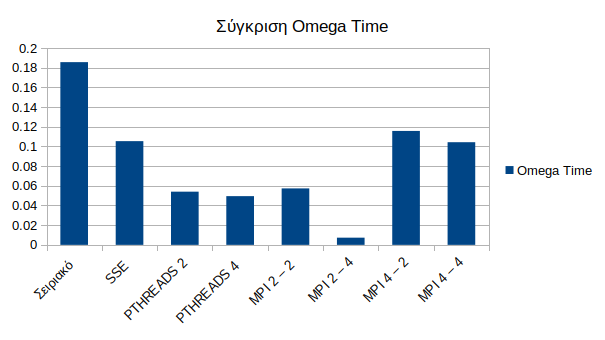
\includegraphics[]{images/first_comp.png}\newline
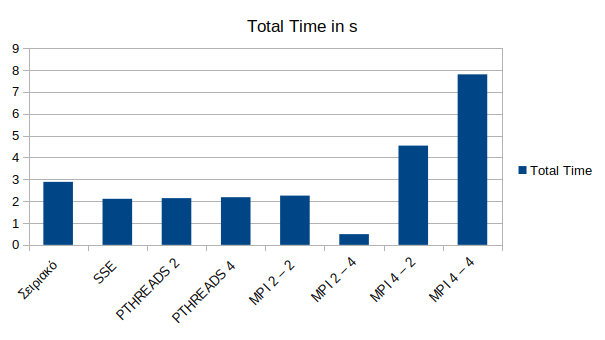
\includegraphics[]{images/sec_comp.png}\newline

\newpage

\section{BONUS 1: MEMORY LAYOUT}
Στο πρώτο κομμάτι από τα bonus μας ζητήθηκε να βελτιώσουμε το memory layout του SSE κωδικά μας. Αρχικά ο χώρος στην μνήμη γίνεται allocate για το κάθε πίνακα ξεχωριστά. Αυτό σημαίνει ότι πρώτα δεσμεύουμε για τον πίνακα 1 τον απαιτούμενο χώρο, δηλαδή δεσμεύουμε για N*sizeof(float),μετά για τον πίνακα 2,μετά για τον πίνακα 3 κτλ. Αυτός ενώ φαίνεται ο σωστότερος και ο προφανής τρόπος δεν είναι ο βέλτιστος. Αυτό συμβαίνει καθώς για να διαχειριστούμε τα δεδομένα μας σε SSE είναι απαραίτητο να τα διαχωρίσουμε σε τετράδες. Οπότε προκύπτει ένα θεμελιώδες πρόβλημα. Κάθε φορά που χρειάζεται να βρούμε δεδομένα από την μνήμη διατρέχουμε μεγάλη απόσταση για να τα βρούμε και να τα χρησιμοποιήσουμε. Για παράδειγμα όταν θέλουμε να χρησιμοποιήσουμε τα LVecss και τα RVecss της πρώτης τετράδας, είναι απαραίτητο να διατρέξουμε όλα τα στοιχεία του LVecss για να φτάσουμε στο RVecss. Αυτό έχει ως αποτέλεσμα να δέχεται πλήγμα τόσο η αποδοτικότητά όσο και η ορθότητα του κώδικα μας. \newline Οπότε τίθεται το ερώτημα πως μπορούμε να το βελτιώσουμε και να γλυτώσουμε αυτά τα περιττά περάσματα της μνήμης. Η λύση που υλοποιήσαμε στο εν λόγω πρόβλημα είναι η εξής. Αντί να δεσμεύουμε τα δεδομένα για τον κάθε πίνακά ξεχωριστά δεσμεύουμε όλα τον πίνακα μαζί. Άρα αντί να κάνουμε 6 malloc, κάνουμε ένα, με μέγεθος N*6*sizeof(float) και αποφασίζουμε να γεμίζουμε τον πίνακα ανά τετράδες. Αυτό σημαίνει ότι από το κελί 0 μέχρι 3 αποθηκεύουμε τις 4 πρώτες τιμές που χρειαζόμαστε για το mVecss,στο 4 με 7 αποθηκεύουμε τις τιμές για το nVecss κτλ. Αυτό έχει ως αποτέλεσμα μετά στο loop μας, που θέλουμε να βελτιώσουμε, όλα τα δεδομένα που είναι απαραίτητα για τις πράξεις να είναι άμεσα προσβάσιμα και δεν χρειάζεται να διατρέξει καμία απόσταση στην μνήμη για να τα βρει. \newline Το πρόβλημα που αντιμετωπίσαμε στην αρχή ήταν ότι όταν γεμίζαμε τον πίνακα με λίγο διαφορετική σειρά από την αρχική της εκφώνησης απέκλιναν τα νούμερα από τα αρχικά οπότε είχαμε λάθος αποτελέσματα. Αυτό επιλύθηκε κρατώντας την αρχική σειρά που μας δόθηκε. Η βελτίωση στην απόδοσή δεν ήταν η αναμενόμενη ούτε με μεγάλο Ν, δηλαδή είχαμε Omega time 1.055113s - Total time 20.977317s για το αρχικό layout ενώ  Omega time 1.054757s - Total time 20.048106s για το βελτιωμένο layout,για  N = 100000000. Είναι πιθανόν να παρατηρήσετε μεγαλύτερη βελτίωση σε ακόμα μεγαλύτερα Ν που όμως δεν μπορούν να τρέξουν οι υπολογιστές μας.\newline


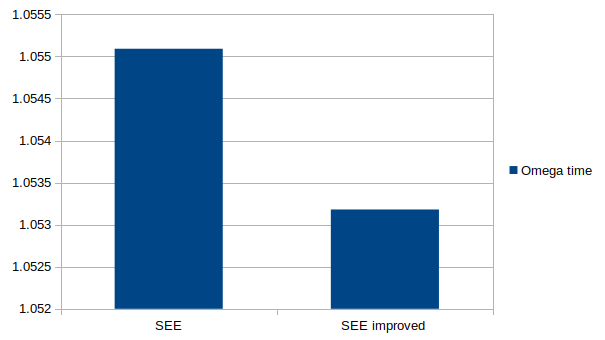
\includegraphics[]{images/first_char_bonus.png}\hspace*{\fill}\newline
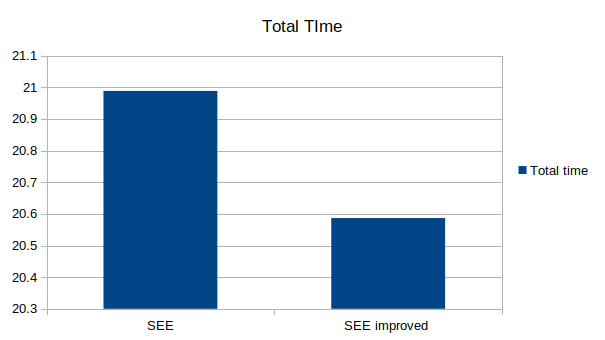
\includegraphics[]{images/second_char_bonus.png}\hspace*{\fill}
\newpage

\section{BONUS 2: LaTeX}
Υλοποιήσαμε την αναφορά του project στο overleaf.com. Σας επισυνάπτουμε τον κώδικα του LaTeX και το pdf.
\end{document}